\section{Introduction}
The purpose of this project is to develop a system to monitor the health of a set of Docker hosts. The structure of such a system is as shown in the figure. 

\begin{figure}[H]
	\begin{subfigure}{\textwidth}
	\centering
		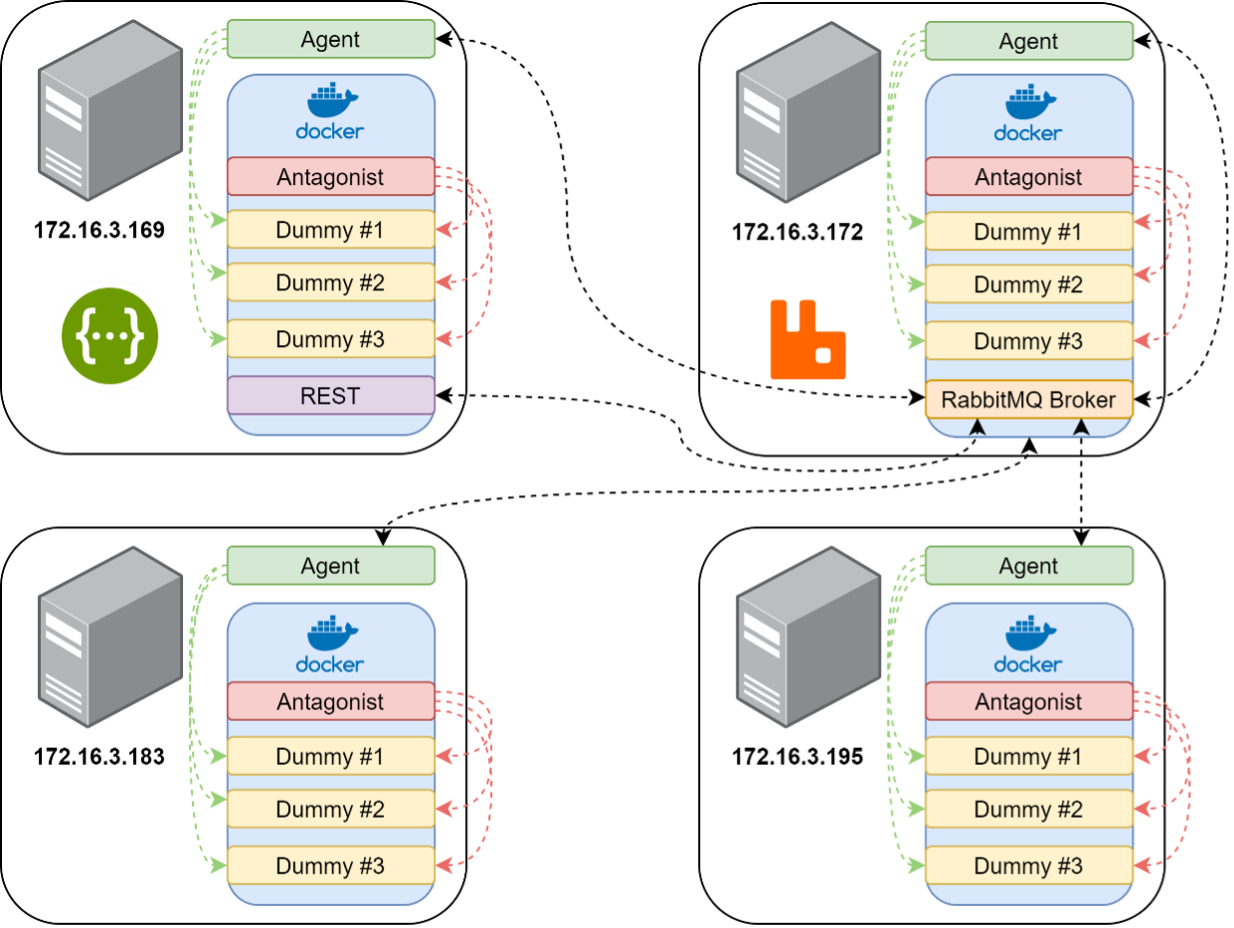
\includegraphics[width=0.9\linewidth]{img/structure.png} 
	\end{subfigure}
\end{figure}

\noindent On each Docker host runs an \textbf{agent}, a software whose task is to periodically check the wellbeing of containers running on the same host. Specifically, every x seconds the agent pings all containers in the \textit{"to be monitored"} list and calculates the experienced packet loss. If a container is down or if it is experiencing packet loss greater than a certain threshold, the agent must destroy it and automatically restart it. 

\noindent The list of containers to be monitored and the threshold are set by the system administrator, who communicates with the system via a \textbf{REST interface}. This interface is exposed by a control module running on one of the Docker hosts (in our case, on the machine with IP address 172.16.3.169).

\noindent In addition, one of the Docker hosts (in our case, the machine with IP address 172.16.3.172) exposes the \textbf{RabbitMQ broker service} as a container, thus allowing the various components (the agents and the swagger server to communicate.

\noindent To test the proper functioning of the system we have:
\begin{itemize}
	\item created "dummy" containers running on each Docker host that will be monitored by each of the agents 
	\item developed the \textbf{antagonist}, a small program running on each Docker host that periodically stops containers or artificially causes packet losses 
\end{itemize}